\chapter{Asking Luxury Shoppers How They Got RICH! (Miami)}

This chapter follows a School of Hard Knocks street interview episode, curated in this volume by LazyingArt LLC. There is no blackboard here, but there is still a quantitative spine. The lecture keeps returning to the same variables until a pattern emerges: peak yearly income, ownership, reinvestment, delegation, patience, and proximity to strong institutions. We will keep the order of the interviews and introduce a small amount of editorial notation only where it helps us preserve the mechanism already present in the spoken material.

\section{Opening Claims and the Scale of the Problem}

The episode opens with a teaser montage. We are given numbers before explanations: one guess of \$750{,}000, one answer of \$8 million, another answer of more than \$2 million, a move from construction to commercial real estate, and a report of assets under management close to a billion dollars. This is not yet a theory. It is the lecturer's way of setting the scale of the unknown.

\begin{equation}
Y_{\max}^{\text{examples}} \in \left\{7.5\times 10^5,\ >2\times 10^6,\ 8\times 10^6\right\}\,\mathrm{USD},
\qquad
M_t \approx 10^9\,\mathrm{USD}.
\end{equation}

What matters is the sequence of questions that accompanies these values. What industry did you choose? Are you a business owner? How much do you manage? What blueprint gets a person to financial freedom? The lecture is telling us from the start that high outcomes will be examined through repeated variables, not through one mystical success story.

A moment later the format is stated plainly: we are in Miami, walking the fashion district, asking visibly successful people how they built their lives. The luxury setting is not the argument. It is the stage on which the argument will be tested.

\section{Medicine Beyond Wages}

The first complete case is the surgeon. The lecture begins with profession and origin before it asks about money. That order matters. We first hear about healthcare, a grandmother from Valencia, Spain, a visit to a surgeon at the age of eight, and then the decision to become a hand surgeon. Only after the work has been grounded in a life story does the lecture ask for the largest yearly income.

The answer is ``in excess of two million,'' but the speaker immediately corrects the listener's likely interpretation. He says, in effect, that the money did not come simply from being paid more and more for surgeries. It came from owning surgery centers, from owning part of the place where the surgery is done, from building a network of orthopedic walk-in centers, and from owning the real estate underneath the operating business.

\begin{definition}
For these notes, the ownership component \(Y_t^{\text{own}}\) means the part of yearly take that arrives because one owns some piece of the platform on which the work is done: the center, the network, the brand, the equity, or the underlying real estate.
\end{definition}

A useful bookkeeping identity, which is not spoken as a formula in the interview but is faithful to its logic, is
\begin{equation}
Y_t = Y_t^{\text{labor}} + Y_t^{\text{own}} + \Delta A_t.
\end{equation}
Here \(Y_t^{\text{labor}}\) is compensation for work, \(Y_t^{\text{own}}\) is business cash flow or distribution from ownership, and \(\Delta A_t\) records gain from productive assets, especially real estate.

\begin{proposition}
If the same professional activity is performed under two arrangements, one pure wage labor and one with ownership of the operating platform, then the second arrangement has a strictly larger ceiling whenever \(Y_t^{\text{own}}+\Delta A_t>0\).
\end{proposition}

\begin{proof}
In the lecture's bookkeeping, the employee receives only \(Y_t^{\text{labor}}\). The owner-operator receives \(Y_t^{\text{labor}} + Y_t^{\text{own}} + \Delta A_t\). If the added terms are positive, then the ceiling rises even though the underlying craft may be the same.
\end{proof}

The surgeon then pushes the point one step further. He says that he learned early that he had to be in his own practice, had to own all the components of it, and had to own the real estate. This is not ornament. It is the central mechanism of the case.

\subsection{Question \& Answer}

The lecture naturally raises a precise question here: why does ownership break the ceiling that labor alone often cannot?

The answer given by the surgeon is very clean. If one works for a large firm, then the firm makes money off one's effort. That may still be a fine arrangement for someone who wants less headache, but it means the margin leaves with the institution. Once one owns the practice, the center, and the building, the margin does not leave. It stays inside the same balance sheet.

We can therefore contrast the two arrangements schematically:
\begin{align}
Y_t^{\text{employee}} &= Y_t^{\text{labor}},\\
Y_t^{\text{owner}} &= Y_t^{\text{labor}} + Y_t^{\text{own}} + \Delta A_t.
\end{align}

The same section of the interview then shifts from production of income to preservation and growth of wealth. Asked for the best financial advice he ever received, the surgeon says: the power of compounding interest. He immediately explains it in plain language: invest early and allow the money to work for you. He also places this beside a rule of restrained consumption. In a luxury district one may enjoy nice things, but when one is young one should be judicious.

A compact update rule consistent with that spoken advice is
\begin{align}
W_{t+1} &= (1+r_t)W_t + S_t,\\
S_t &= Y_t - C_t,\\
C_t &= C_t^{\text{needs}} + C_t^{\text{wants}}.
\end{align}
Here \(W_t\) is investable wealth, \(r_t\) is the return on that wealth, \(S_t\) is the fresh contribution made out of current income, and consumption is split into basic spending and discretionary spending.

\paragraph{Worked update.}
If we momentarily freeze the return and the fresh contribution so that \(r_t=r\) and \(S_t=S\), then two periods of the update already show the mechanism:
\begin{align}
W_1 &= (1+r)W_0 + S,\\
W_2 &= (1+r)W_1 + S \\
&= (1+r)^2W_0 + \bigl[(1+r)+1\bigr]S.
\end{align}
The point is simple but decisive: the old wealth compounds, and the new contributions accumulate on top of that compounding base. This is exactly the structure the surgeon wants his son to learn.

\paragraph{Editorial schematic.}
The lecture never draws the following picture, but it captures the movement we have just been shown in words.

\begin{figure}
\centering
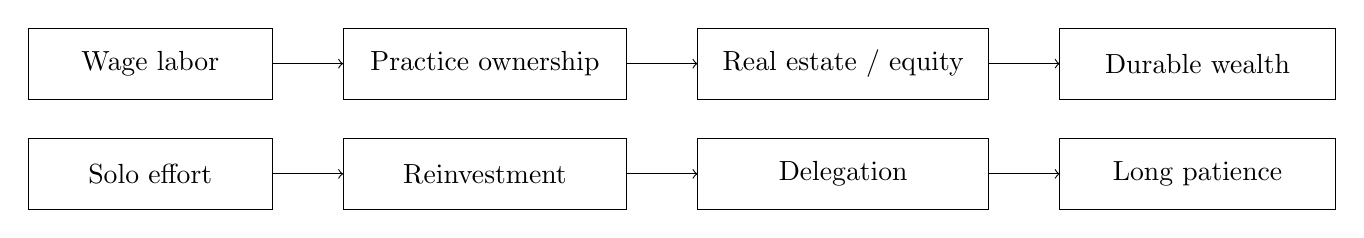
\begin{tikzpicture}[x=1cm,y=1cm]
\draw (0,0) rectangle (3.1,0.9);
\node at (1.55,0.45) {Wage labor};
\draw[->] (3.1,0.45) -- (4.0,0.45);
\draw (4.0,0) rectangle (7.6,0.9);
\node at (5.8,0.45) {Practice ownership};
\draw[->] (7.6,0.45) -- (8.5,0.45);
\draw (8.5,0) rectangle (12.2,0.9);
\node at (10.35,0.45) {Real estate / equity};
\draw[->] (12.2,0.45) -- (13.1,0.45);
\draw (13.1,0) rectangle (16.6,0.9);
\node at (14.85,0.45) {Durable wealth};

\draw (0,-1.4) rectangle (3.1,-0.5);
\node at (1.55,-0.95) {Solo effort};
\draw[->] (3.1,-0.95) -- (4.0,-0.95);
\draw (4.0,-1.4) rectangle (7.6,-0.5);
\node at (5.8,-0.95) {Reinvestment};
\draw[->] (7.6,-0.95) -- (8.5,-0.95);
\draw (8.5,-1.4) rectangle (12.2,-0.5);
\node at (10.35,-0.95) {Delegation};
\draw[->] (12.2,-0.95) -- (13.1,-0.95);
\draw (13.1,-1.4) rectangle (16.6,-0.5);
\node at (14.85,-0.95) {Long patience};
\end{tikzpicture}
\end{figure}

The first interview therefore gives us the deepest early lesson of the chapter. Skill matters. But wealth, at scale, appears when skill is wrapped inside ownership.

\section{Luck, Product Discovery, and the Cost of Growth}

The lecture then breathes. There is a warm interruption from a fan from Argentina, a burst of repeated thank-yous in the transcript, and then a slightly garbled return to business advice. We should not smooth this away too much. The street rhythm matters. The lecture is not presenting a polished seminar; it is harvesting principles in public.

The next partially preserved voice says he got lucky. He would like to say he was brilliant, but instead he says he went to a seminar, saw a product, saw a need in the market, noticed that nobody was doing it, and decided to take a chance. The striking maxim that follows is baseball-shaped rather than algebraic: one does not hit a home run without taking many swings. Even in its roughness, this is a statement about repeated trials and asymmetric upside.

A related speaker then says something even more compact: finance is not about math, it is about choices. The key opposition is between needs and wants. We may have every want in the world, but we must first deal with what is necessary and only then climb outward from that base.

The contractor who follows gives the same lesson in harder operational language. He has been in the industry for twenty-seven years, began with his father, and insists that the secret to sales is to produce a perfect product. If the work is great, the clients find you. But he pairs this with another rule that can sound reckless if taken carelessly: one must spend money to make money. What he means is not blind expenditure. He means that tools, labor, and team quality are themselves productive inputs.

A cautious update rule for that spoken logic is
\begin{equation}
K_{t+1} = K_t + I_t - \delta K_t.
\end{equation}
Here \(K_t\) is productive capacity in a broad sense, \(I_t\) is reinvestment, and \(\delta K_t\) represents wear, drift, or simple obsolescence.

\paragraph{Operational reading.}
\begin{enumerate}
\item If extra cash is consumed immediately, then productive capacity does not rise.
\item If part of the surplus is redirected into \(I_t\), then \(K_t\) increases.
\item Better tools and better labor increase what the firm can promise and what it can reliably deliver.
\item Better delivery feeds future revenue, which then funds further reinvestment.
\end{enumerate}

This is the place in the lecture where a simplistic morality of thrift is quietly corrected. Earlier we were told not to confuse luxury with wisdom. Here we are told not to confuse frugality with growth. Some money must be withheld from consumption. Some money must be driven back into the business machine.

\section{Finance at Scale: Delegation, Risk Narratives, and Sales}

The next cleanly recorded case is finance in a more literal street-business sense: mortgage, personal loans, credit cards. ``We lend out money,'' the speaker says. He has owned the business for about twenty years, always wanted to be his own boss, and reports a single-year income of about \$8 million. This is the sharpest scale jump in the middle of the episode, and the lecturer immediately asks the right follow-up: what takes a person from six figures to seven?

\subsection{Question \& Answer}

The answer now shifts the chapter from ownership to scaling. Work hard, yes. But more importantly, learn to delegate. Learn to trust other people to do the job. The speaker explicitly names the founder's trap: ``I can do it myself.'' The lecture rejects that instinct as a ceiling.

A compact way to represent the claim is
\begin{equation}
Q_t = q(K_t,n_t), \qquad Q_t^{\text{delegated}} > Q_t^{\text{solo}}.
\end{equation}
Here \(Q_t\) is output or scalable business throughput, \(K_t\) is productive capacity, and \(n_t\) is effective team span. The claim is not that delegation is magic. It is that the one-person ceiling can be broken only by trusted multiplication of effort.

The speaker then gives the practical version. If one is responsible to other people and can trust them, one can grow to hundreds, perhaps thousands, of employees. We should hear this as an extension of the earlier surgeon case. Ownership enlarges the claim on margin. Delegation enlarges the capacity that produces margin.

The same interview then turns to investment advice. The speaker strongly recommends crypto and frames it as a control question: in his telling, the bank controls your money when it sits in the bank, whereas crypto is yours in a more direct way.

\begin{remark}
The chapter should preserve the structure of this claim---delegated custody versus direct control---but should not elevate the numerical threshold mentioned in the interview or the legal absolutes that follow into settled doctrine. The important thing here is the speaker's risk narrative, not the final truth of the policy details.
\end{remark}

The interview closes with a shift from investment back to client acquisition.

\subsection{Question \& Answer}

Asked how one consistently lands clients, the speaker gives a surprisingly general answer: sales is everywhere. A doctor sells, an attorney sells, a dentist sells, and therefore sales is not a narrow profession but a universal layer of economic life. That answer matters because it changes the question. We are no longer asking for one clever closing trick. We are asking how one learns to inhabit a world in which every exchange involves persuasion, trust, and presentation.

The speaker's concrete prescription is apprenticeship. Find the top producer in the company and sit next to that person. That is the interview's version of local training under a master operator. The lecture has now repeated a motif we will see again: do not merely admire successful people from afar; place yourself in their working radius.

At this point the episode inserts a sponsor intermission about meals, time, routine, and entrepreneurial efficiency. We should register it as a structural pause rather than as part of the chapter's core argument. Still, even the pause keeps one rhetorical thread alive: time is scarce, and successful people protect their productive hours.

\section{Career Capital in Luxury and Hospitality}

After the sponsor break the lecture returns to the street, but the tone changes. We are now in hospitality, wines, and spirits. The speaker says it took twenty years to get into the shoes he now occupies, and now, as a part partner or minority stakeholder in the brand, he is in one sense back where he started: selling account by account, bottle by bottle.

That reversal is instructive. The lecture is telling us that ownership is not an escape from work. It is a transformation of work. The speaker says the real work begins where others end. The sale is not the finish line. If one owns a small business, one must roll up one's sleeves and perform the rest of the chain.

This case also widens the book's notion of capital. The speaker worked for Louis Vuitton and other French conglomerates before building toward ownership. He advises the listener to inspect not just salary, but the whole package: features, benefits, growth opportunities, equity, and, most importantly, the quality of the boss. A useful bookkeeping line, not spoken verbatim but faithful to the structure of the advice, is
\begin{equation}
Y_t^{\text{career}} = Y_t^{\text{salary}} + Y_t^{\text{bonus}} + Y_t^{\text{equity}} + Y_t^{\text{optionality}}.
\end{equation}
Here the last term means future career leverage: experience, institutional pedigree, exposure to larger operators, and access to better future positions.

The lecture's point is not merely that one should choose jobs with more pay. It is that one should choose trajectories with better curvature. We may summarize the package logic as follows:
\begin{itemize}
\item present cash compensation,
\item future growth inside the organization,
\item equity or ownership opportunities,
\item the training value of the people above us.
\end{itemize}

The speaker says he worked with industry titans, multiple billionaires, and that the experience gained there could not be replicated in a lifetime by ordinary means. This is another way of naming capital. Not only financial capital, but career capital, institutional capital, and reputational capital.

\section{Todd Napola and the Billion-Dollar Horizon}

The lecture now announces a ``special surprise'' and leaves the casual street sweep for a more deliberate capstone interview with Todd Napola. The shift in tone is immediate. We move from luxury shoppers to a commercial real estate founder who manages roughly a billion dollars of property and client assets.

\begin{equation}
M_t \approx 10^9\,\mathrm{USD}, \qquad \tau_{\text{decision}}^{\text{RE}} \gg 1\ \text{day}.
\end{equation}

The second expression is our shorthand for the central real-estate lesson that follows. Napola says real estate is not like staring at an E-Trade account every day. Values move, but the operative horizon is not daily fluctuation. It is multi-year, even generational patience. The richest real-estate families look generational because they began buying a hundred years ago, but the lesson drawn is not passive admiration. It is that one must be the one who starts now.

The lecture then changes register once again and asks about the difference between the middle class and the wealthy. Napola's answer is not gentle. He says the middle class got stuck inside an inherited script that no longer works. In compressed form, the obsolete script is
\begin{itemize}
\item go to school,
\item get a good job,
\item save money,
\item buy a house,
\item pay it off,
\item retire on a pension.
\end{itemize}
His argument is that this story was sold to older generations under historical conditions that no longer obtain. The result is a class that bears obligations without either the subsidies of poverty or the privileges of wealth.

This is the broadest sociological move in the lecture, but it is still linked to the same economic mechanism. If the old script does not produce independence, then one must move toward value creation, ownership, and long-horizon assets.

\subsection{Question \& Answer}

The final and clearest question of the episode is the one the teaser promised at the beginning: what is the blueprint for becoming a millionaire and getting serious about financial freedom?

Napola's answer is remarkably disciplined. Work hard to add value to other people. Place yourself near very wealthy people, not because wealth is magical, but because proximity destroys the illusion that they are made of different material. He gives a concrete operational example: tell a great salesperson who feels alien to wealth to work as a valet at a country club. After three months he learns that rich people tell the same jokes and wear the same kinds of things. The metaphysical barrier drops. Then one can ask the real question: where can I add value?

The answer is therefore not mere positive thinking. It has three stages.
\begin{enumerate}
\item First, remove the false transcendence of wealth.
\item Second, identify where value can be added.
\item Third, model people who came from the bottom and already built the path.
\end{enumerate}

\begin{proposition}
In the lecture's final synthesis, wealth is most likely to accumulate when value creation, ownership, and patience are placed inside the orbit of already successful operators.
\end{proposition}

\begin{proof}
The closing interview combines three claims. One must add value rather than merely seek status. One must get near people who already allocate capital at scale. And one must wait on a horizon long enough for ownership to matter. Each claim enlarges the base from which future gains are drawn; together they form the lecture's strongest blueprint.
\end{proof}

\section{Summary}

The chapter begins with spectacle but does not end there. Across medicine, contracting, finance, hospitality, and commercial real estate, the same structure returns. Large yearly income is not the whole story. What matters is the decomposition of income into labor, ownership, and asset gain; the treatment of surplus through reinvestment and compounding; the escape from the one-person ceiling through delegation; and the discipline to choose long horizons over daily noise.

If we compress the full lecture into one line, it is this: labor may start the machine, but ownership, reinvestment, delegation, and patience determine whether the machine ever becomes wealth.